\documentclass[11pt]{scrartcl}

\usepackage{fontspec}
\setmainfont{STIX}
%\setmainfont{EB Garamond}
%\setmainfont{Comic Neue}
%\setsansfont{Comic Sans MS}

\usepackage{polyglossia}
\setdefaultlanguage{english}

\usepackage[margin=2.5cm,bottom=3cm]{geometry}

\setlength\parskip{0.5ex}

\usepackage{enumitem}
\setlist{noitemsep,topsep=1ex,parsep=0.25ex,partopsep=0pt}

\usepackage{tikz}
\usetikzlibrary{positioning}
\usetikzlibrary{calc}

\usepackage{amssymb}

\usepackage[export]{adjustbox}
\usepackage{graphicx}
\usepackage{float}
\usepackage{blindtext}
\usepackage[colorlinks=true]{hyperref}
\newcommand{\cminlinett}[1]{\texttt{#1}}
\usepackage{listings}
\lstset{
	basicstyle=\ttfamily,
	breaklines=true,
	breakatwhitespace=true,
	tabsize=5,
	extendedchars=true,
	inputencoding=utf8,
	showstringspaces=false,
	texcl=false,
	captionpos=b,
	columns=fullflexible
}
\newcommand{\commonmarkimage}[2]{
\begin{figure}[H]
	\centering
	\includegraphics[max width=\linewidth]{#1}
	\caption{#2}
\end{figure}
}

\newcommand{\enq}[1]{«#1»}

\author{Dominik Schmidt \textsf{schmidom@student.ethz.ch}}
\title{Scientific Software Management with Gentoo Linux}
\date{\today}

\newcommand{\dg}[1]{\texttt{#1}}

\begin{document}
	\maketitle
	\begin{abstract}
		In this document key problems and approaches in scientific
		software management with Gentoo Linux are discussed.
		In particular, the \dg{.gentoo} standard, a method to distribute software dependencies with publications and projects, is introduced.
		This method is then applied to multiple use-cases, including:
		single-purpose-machines\footnote{Docker, Travis CI},
		scientific computing clusters\footnote{Local compute machines, the EULER cluster}
		and virtual machines\footnote{OpenStack}
	\end{abstract}
	\section{Introduction}
		Current empirical research is generally - and particularly in the case of neuroscience - contingent on the execution of complex software pipelines for modeling and statistical analysis (e.g. General Linear Modelling, Independent Component Analysis, etc.).
		The software needed to execute and dynamically construct such pipelines, in turn relies on more software, generally resulting in a very large dependency graph.
		Trees do not suffice, since the dependencies will most likely contain loops, even for simple programs. A basic example are C compilers, that depend on an already compiled libc, forming the cycle compiler $\leftrightarrows$ libc.

		\begin{figure}[H]
			\centering
			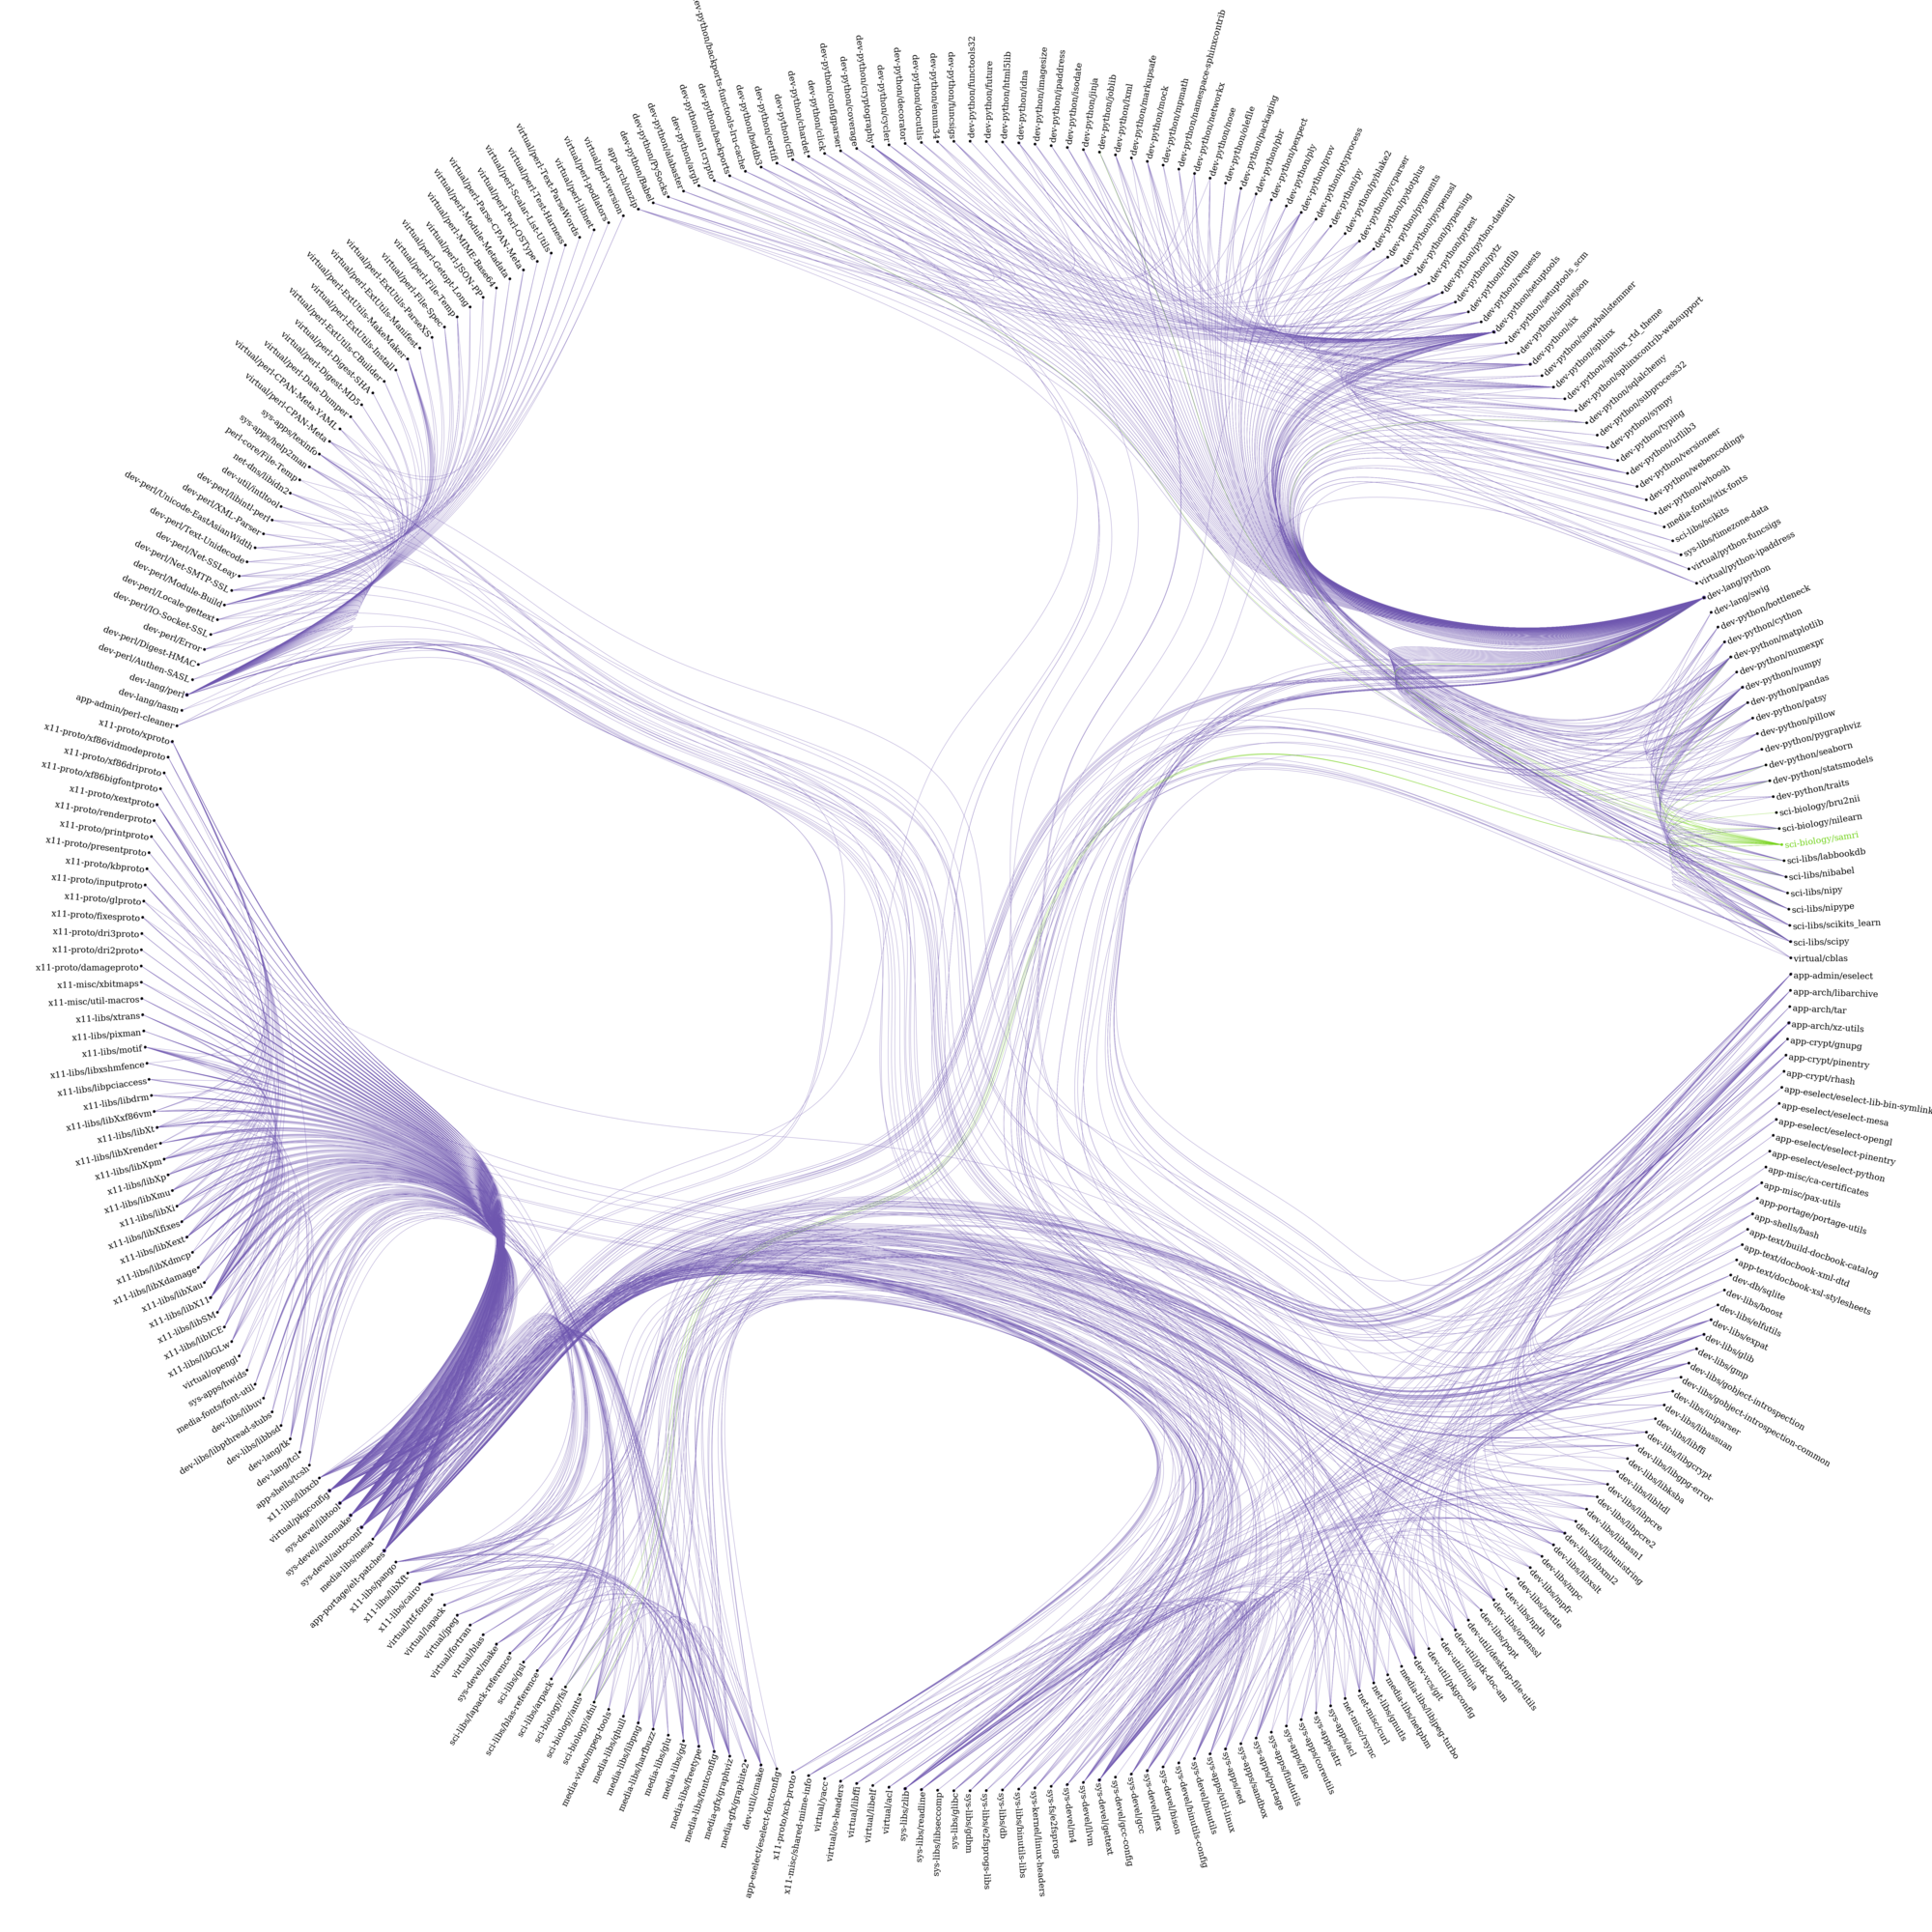
\includegraphics[width=0.75\linewidth]{graph/Real_Dependencygraph/RealDepgraph2.png}
			\caption{An actual dependency graph of the SAMRI package developed at the Institute for Biomedical Technology (IBT). The green lines in the upper right corner connect SAMRI to its direct dependency packages.}
		\end{figure}
		
		Hence, package managers are employed to do the dependency resolution.
		One such package managers is Portage, used by Gentoo Linux and derivatives.
		Its key-feature are source-based packages, i.e. packages not based on pre-compiled binary archives but on recipes (called Ebuilds), which specify how to obtain, build, and test the software, as well as what other packages it depends on.
		This source-based approach is characterized by a number of advantages:
		\begin{enumerate}
			\item Ebuilds are easy to write, since they are straight-forward text files written in Bash, conforming to well-documented standards.
			\item Ebuilds are usually easily updated to a new version just by incrementing the version number in the Ebuild file name.
			\item Ebuilds allow for a better integration of live and pre-release packages, facilitating access to the most recent code versions.
			This allows for better upstreaming of user patches, since the user is working on the same version as the developers.
			\item The resulting programs are optimized by the compiler to run as efficiently as possible on the machine they are deployed on\footnote{Binary distributions like Debian Linux have binaries compiled to run reasonably fast on \emph{all} machines, which might not always be the fastest way for your specific machine}
		\end{enumerate}
		
		To make this Gentoo Linux approach more suitable for scientific software, we designed a way of distributing live Ebuilds alongside the software they package (the .gentoo standard) - as opposed to the canonical distribution via an overlay - and applied this standard to multiple use cases.
	\input{DotGentoo.tex}
	\input{UseCases.tex}
	\input{BuildServer.tex}
	\input{BLAS_Lapack.tex}
	\appendix
	\input{BuildServerExamples.tex}
\end{document}
